\documentclass[twoside]{article}

\usepackage{aistats2024}
% If your paper is accepted, change the options for the package
% aistats2022 as follows:
%
%\usepackage[accepted]{aistats2024}
%
% This option will print headings for the title of your paper and
% headings for the authors names, plus a copyright note at the end of
% the first column of the first page.

% If you set papersize explicitly, activate the following three lines:
%\special{papersize = 8.5in, 11in}
%\setlength{\pdfpageheight}{11in}
%\setlength{\pdfpagewidth}{8.5in}

% If you use natbib package, activate the following three lines:
%\usepackage[round]{natbib}
%\renewcommand{\bibname}{References}
%\renewcommand{\bibsection}{\subsubsection*{\bibname}}

% If you use BibTeX in apalike style, activate the following line:
%\bibliographystyle{apalike}

%%%%% NEW MATH DEFINITIONS %%%%%

\usepackage{amsmath,amsfonts,bm}

% Mark sections of captions for referring to divisions of figures
\newcommand{\figleft}{{\em (Left)}}
\newcommand{\figcenter}{{\em (Center)}}
\newcommand{\figright}{{\em (Right)}}
\newcommand{\figtop}{{\em (Top)}}
\newcommand{\figbottom}{{\em (Bottom)}}
\newcommand{\captiona}{{\em (a)}}
\newcommand{\captionb}{{\em (b)}}
\newcommand{\captionc}{{\em (c)}}
\newcommand{\captiond}{{\em (d)}}

% Highlight a newly defined term
\newcommand{\newterm}[1]{{\bf #1}}


% Figure reference, lower-case.
\def\figref#1{figure~\ref{#1}}
% Figure reference, capital. For start of sentence
\def\Figref#1{Figure~\ref{#1}}
\def\twofigref#1#2{figures \ref{#1} and \ref{#2}}
\def\quadfigref#1#2#3#4{figures \ref{#1}, \ref{#2}, \ref{#3} and \ref{#4}}
% Section reference, lower-case.
\def\secref#1{section~\ref{#1}}
% Section reference, capital.
\def\Secref#1{Section~\ref{#1}}
% Reference to two sections.
\def\twosecrefs#1#2{sections \ref{#1} and \ref{#2}}
% Reference to three sections.
\def\secrefs#1#2#3{sections \ref{#1}, \ref{#2} and \ref{#3}}
% Reference to an equation, lower-case.
\def\eqref#1{equation~\ref{#1}}
% Reference to an equation, upper case
\def\Eqref#1{Equation~\ref{#1}}
% A raw reference to an equation---avoid using if possible
\def\plaineqref#1{\ref{#1}}
% Reference to a chapter, lower-case.
\def\chapref#1{chapter~\ref{#1}}
% Reference to an equation, upper case.
\def\Chapref#1{Chapter~\ref{#1}}
% Reference to a range of chapters
\def\rangechapref#1#2{chapters\ref{#1}--\ref{#2}}
% Reference to an algorithm, lower-case.
\def\algref#1{algorithm~\ref{#1}}
% Reference to an algorithm, upper case.
\def\Algref#1{Algorithm~\ref{#1}}
\def\twoalgref#1#2{algorithms \ref{#1} and \ref{#2}}
\def\Twoalgref#1#2{Algorithms \ref{#1} and \ref{#2}}
% Reference to a part, lower case
\def\partref#1{part~\ref{#1}}
% Reference to a part, upper case
\def\Partref#1{Part~\ref{#1}}
\def\twopartref#1#2{parts \ref{#1} and \ref{#2}}

\def\ceil#1{\lceil #1 \rceil}
\def\floor#1{\lfloor #1 \rfloor}
\def\1{\bm{1}}
\newcommand{\train}{\mathcal{D}}
\newcommand{\valid}{\mathcal{D_{\mathrm{valid}}}}
\newcommand{\test}{\mathcal{D_{\mathrm{test}}}}

\def\eps{{\epsilon}}


% Random variables
\def\reta{{\textnormal{$\eta$}}}
\def\ra{{\textnormal{a}}}
\def\rb{{\textnormal{b}}}
\def\rc{{\textnormal{c}}}
\def\rd{{\textnormal{d}}}
\def\re{{\textnormal{e}}}
\def\rf{{\textnormal{f}}}
\def\rg{{\textnormal{g}}}
\def\rh{{\textnormal{h}}}
\def\ri{{\textnormal{i}}}
\def\rj{{\textnormal{j}}}
\def\rk{{\textnormal{k}}}
\def\rl{{\textnormal{l}}}
% rm is already a command, just don't name any random variables m
\def\rn{{\textnormal{n}}}
\def\ro{{\textnormal{o}}}
\def\rp{{\textnormal{p}}}
\def\rq{{\textnormal{q}}}
\def\rr{{\textnormal{r}}}
\def\rs{{\textnormal{s}}}
\def\rt{{\textnormal{t}}}
\def\ru{{\textnormal{u}}}
\def\rv{{\textnormal{v}}}
\def\rw{{\textnormal{w}}}
\def\rx{{\textnormal{x}}}
\def\ry{{\textnormal{y}}}
\def\rz{{\textnormal{z}}}

% Random vectors
\def\rvepsilon{{\mathbf{\epsilon}}}
\def\rvtheta{{\mathbf{\theta}}}
\def\rva{{\mathbf{a}}}
\def\rvb{{\mathbf{b}}}
\def\rvc{{\mathbf{c}}}
\def\rvd{{\mathbf{d}}}
\def\rve{{\mathbf{e}}}
\def\rvf{{\mathbf{f}}}
\def\rvg{{\mathbf{g}}}
\def\rvh{{\mathbf{h}}}
\def\rvu{{\mathbf{i}}}
\def\rvj{{\mathbf{j}}}
\def\rvk{{\mathbf{k}}}
\def\rvl{{\mathbf{l}}}
\def\rvm{{\mathbf{m}}}
\def\rvn{{\mathbf{n}}}
\def\rvo{{\mathbf{o}}}
\def\rvp{{\mathbf{p}}}
\def\rvq{{\mathbf{q}}}
\def\rvr{{\mathbf{r}}}
\def\rvs{{\mathbf{s}}}
\def\rvt{{\mathbf{t}}}
\def\rvu{{\mathbf{u}}}
\def\rvv{{\mathbf{v}}}
\def\rvw{{\mathbf{w}}}
\def\rvx{{\mathbf{x}}}
\def\rvy{{\mathbf{y}}}
\def\rvz{{\mathbf{z}}}

% Elements of random vectors
\def\erva{{\textnormal{a}}}
\def\ervb{{\textnormal{b}}}
\def\ervc{{\textnormal{c}}}
\def\ervd{{\textnormal{d}}}
\def\erve{{\textnormal{e}}}
\def\ervf{{\textnormal{f}}}
\def\ervg{{\textnormal{g}}}
\def\ervh{{\textnormal{h}}}
\def\ervi{{\textnormal{i}}}
\def\ervj{{\textnormal{j}}}
\def\ervk{{\textnormal{k}}}
\def\ervl{{\textnormal{l}}}
\def\ervm{{\textnormal{m}}}
\def\ervn{{\textnormal{n}}}
\def\ervo{{\textnormal{o}}}
\def\ervp{{\textnormal{p}}}
\def\ervq{{\textnormal{q}}}
\def\ervr{{\textnormal{r}}}
\def\ervs{{\textnormal{s}}}
\def\ervt{{\textnormal{t}}}
\def\ervu{{\textnormal{u}}}
\def\ervv{{\textnormal{v}}}
\def\ervw{{\textnormal{w}}}
\def\ervx{{\textnormal{x}}}
\def\ervy{{\textnormal{y}}}
\def\ervz{{\textnormal{z}}}

% Random matrices
\def\rmA{{\mathbf{A}}}
\def\rmB{{\mathbf{B}}}
\def\rmC{{\mathbf{C}}}
\def\rmD{{\mathbf{D}}}
\def\rmE{{\mathbf{E}}}
\def\rmF{{\mathbf{F}}}
\def\rmG{{\mathbf{G}}}
\def\rmH{{\mathbf{H}}}
\def\rmI{{\mathbf{I}}}
\def\rmJ{{\mathbf{J}}}
\def\rmK{{\mathbf{K}}}
\def\rmL{{\mathbf{L}}}
\def\rmM{{\mathbf{M}}}
\def\rmN{{\mathbf{N}}}
\def\rmO{{\mathbf{O}}}
\def\rmP{{\mathbf{P}}}
\def\rmQ{{\mathbf{Q}}}
\def\rmR{{\mathbf{R}}}
\def\rmS{{\mathbf{S}}}
\def\rmT{{\mathbf{T}}}
\def\rmU{{\mathbf{U}}}
\def\rmV{{\mathbf{V}}}
\def\rmW{{\mathbf{W}}}
\def\rmX{{\mathbf{X}}}
\def\rmY{{\mathbf{Y}}}
\def\rmZ{{\mathbf{Z}}}

% Elements of random matrices
\def\ermA{{\textnormal{A}}}
\def\ermB{{\textnormal{B}}}
\def\ermC{{\textnormal{C}}}
\def\ermD{{\textnormal{D}}}
\def\ermE{{\textnormal{E}}}
\def\ermF{{\textnormal{F}}}
\def\ermG{{\textnormal{G}}}
\def\ermH{{\textnormal{H}}}
\def\ermI{{\textnormal{I}}}
\def\ermJ{{\textnormal{J}}}
\def\ermK{{\textnormal{K}}}
\def\ermL{{\textnormal{L}}}
\def\ermM{{\textnormal{M}}}
\def\ermN{{\textnormal{N}}}
\def\ermO{{\textnormal{O}}}
\def\ermP{{\textnormal{P}}}
\def\ermQ{{\textnormal{Q}}}
\def\ermR{{\textnormal{R}}}
\def\ermS{{\textnormal{S}}}
\def\ermT{{\textnormal{T}}}
\def\ermU{{\textnormal{U}}}
\def\ermV{{\textnormal{V}}}
\def\ermW{{\textnormal{W}}}
\def\ermX{{\textnormal{X}}}
\def\ermY{{\textnormal{Y}}}
\def\ermZ{{\textnormal{Z}}}

% Vectors
\def\vzero{{\bm{0}}}
\def\vone{{\bm{1}}}
\def\vmu{{\bm{\mu}}}
\def\vtheta{{\bm{\theta}}}
\def\va{{\bm{a}}}
\def\vb{{\bm{b}}}
\def\vc{{\bm{c}}}
\def\vd{{\bm{d}}}
\def\ve{{\bm{e}}}
\def\vf{{\bm{f}}}
\def\vg{{\bm{g}}}
\def\vh{{\bm{h}}}
\def\vi{{\bm{i}}}
\def\vj{{\bm{j}}}
\def\vk{{\bm{k}}}
\def\vl{{\bm{l}}}
\def\vm{{\bm{m}}}
\def\vn{{\bm{n}}}
\def\vo{{\bm{o}}}
\def\vp{{\bm{p}}}
\def\vq{{\bm{q}}}
\def\vr{{\bm{r}}}
\def\vs{{\bm{s}}}
\def\vt{{\bm{t}}}
\def\vu{{\bm{u}}}
\def\vv{{\bm{v}}}
\def\vw{{\bm{w}}}
\def\vx{{\bm{x}}}
\def\vy{{\bm{y}}}
\def\vz{{\bm{z}}}

% Elements of vectors
\def\evalpha{{\alpha}}
\def\evbeta{{\beta}}
\def\evepsilon{{\epsilon}}
\def\evlambda{{\lambda}}
\def\evomega{{\omega}}
\def\evmu{{\mu}}
\def\evpsi{{\psi}}
\def\evsigma{{\sigma}}
\def\evtheta{{\theta}}
\def\eva{{a}}
\def\evb{{b}}
\def\evc{{c}}
\def\evd{{d}}
\def\eve{{e}}
\def\evf{{f}}
\def\evg{{g}}
\def\evh{{h}}
\def\evi{{i}}
\def\evj{{j}}
\def\evk{{k}}
\def\evl{{l}}
\def\evm{{m}}
\def\evn{{n}}
\def\evo{{o}}
\def\evp{{p}}
\def\evq{{q}}
\def\evr{{r}}
\def\evs{{s}}
\def\evt{{t}}
\def\evu{{u}}
\def\evv{{v}}
\def\evw{{w}}
\def\evx{{x}}
\def\evy{{y}}
\def\evz{{z}}

% Matrix
\def\mA{{\bm{A}}}
\def\mB{{\bm{B}}}
\def\mC{{\bm{C}}}
\def\mD{{\bm{D}}}
\def\mE{{\bm{E}}}
\def\mF{{\bm{F}}}
\def\mG{{\bm{G}}}
\def\mH{{\bm{H}}}
\def\mI{{\bm{I}}}
\def\mJ{{\bm{J}}}
\def\mK{{\bm{K}}}
\def\mL{{\bm{L}}}
\def\mM{{\bm{M}}}
\def\mN{{\bm{N}}}
\def\mO{{\bm{O}}}
\def\mP{{\bm{P}}}
\def\mQ{{\bm{Q}}}
\def\mR{{\bm{R}}}
\def\mS{{\bm{S}}}
\def\mT{{\bm{T}}}
\def\mU{{\bm{U}}}
\def\mV{{\bm{V}}}
\def\mW{{\bm{W}}}
\def\mX{{\bm{X}}}
\def\mY{{\bm{Y}}}
\def\mZ{{\bm{Z}}}
\def\mBeta{{\bm{\beta}}}
\def\mPhi{{\bm{\Phi}}}
\def\mLambda{{\bm{\Lambda}}}
\def\mSigma{{\bm{\Sigma}}}

% Tensor
\DeclareMathAlphabet{\mathsfit}{\encodingdefault}{\sfdefault}{m}{sl}
\SetMathAlphabet{\mathsfit}{bold}{\encodingdefault}{\sfdefault}{bx}{n}
\newcommand{\tens}[1]{\bm{\mathsfit{#1}}}
\def\tA{{\tens{A}}}
\def\tB{{\tens{B}}}
\def\tC{{\tens{C}}}
\def\tD{{\tens{D}}}
\def\tE{{\tens{E}}}
\def\tF{{\tens{F}}}
\def\tG{{\tens{G}}}
\def\tH{{\tens{H}}}
\def\tI{{\tens{I}}}
\def\tJ{{\tens{J}}}
\def\tK{{\tens{K}}}
\def\tL{{\tens{L}}}
\def\tM{{\tens{M}}}
\def\tN{{\tens{N}}}
\def\tO{{\tens{O}}}
\def\tP{{\tens{P}}}
\def\tQ{{\tens{Q}}}
\def\tR{{\tens{R}}}
\def\tS{{\tens{S}}}
\def\tT{{\tens{T}}}
\def\tU{{\tens{U}}}
\def\tV{{\tens{V}}}
\def\tW{{\tens{W}}}
\def\tX{{\tens{X}}}
\def\tY{{\tens{Y}}}
\def\tZ{{\tens{Z}}}


% Graph
\def\gA{{\mathcal{A}}}
\def\gB{{\mathcal{B}}}
\def\gC{{\mathcal{C}}}
\def\gD{{\mathcal{D}}}
\def\gE{{\mathcal{E}}}
\def\gF{{\mathcal{F}}}
\def\gG{{\mathcal{G}}}
\def\gH{{\mathcal{H}}}
\def\gI{{\mathcal{I}}}
\def\gJ{{\mathcal{J}}}
\def\gK{{\mathcal{K}}}
\def\gL{{\mathcal{L}}}
\def\gM{{\mathcal{M}}}
\def\gN{{\mathcal{N}}}
\def\gO{{\mathcal{O}}}
\def\gP{{\mathcal{P}}}
\def\gQ{{\mathcal{Q}}}
\def\gR{{\mathcal{R}}}
\def\gS{{\mathcal{S}}}
\def\gT{{\mathcal{T}}}
\def\gU{{\mathcal{U}}}
\def\gV{{\mathcal{V}}}
\def\gW{{\mathcal{W}}}
\def\gX{{\mathcal{X}}}
\def\gY{{\mathcal{Y}}}
\def\gZ{{\mathcal{Z}}}

% Sets
\def\sA{{\mathbb{A}}}
\def\sB{{\mathbb{B}}}
\def\sC{{\mathbb{C}}}
\def\sD{{\mathbb{D}}}
% Don't use a set called E, because this would be the same as our symbol
% for expectation.
\def\sF{{\mathbb{F}}}
\def\sG{{\mathbb{G}}}
\def\sH{{\mathbb{H}}}
\def\sI{{\mathbb{I}}}
\def\sJ{{\mathbb{J}}}
\def\sK{{\mathbb{K}}}
\def\sL{{\mathbb{L}}}
\def\sM{{\mathbb{M}}}
\def\sN{{\mathbb{N}}}
\def\sO{{\mathbb{O}}}
\def\sP{{\mathbb{P}}}
\def\sQ{{\mathbb{Q}}}
\def\sR{{\mathbb{R}}}
\def\sS{{\mathbb{S}}}
\def\sT{{\mathbb{T}}}
\def\sU{{\mathbb{U}}}
\def\sV{{\mathbb{V}}}
\def\sW{{\mathbb{W}}}
\def\sX{{\mathbb{X}}}
\def\sY{{\mathbb{Y}}}
\def\sZ{{\mathbb{Z}}}

% Entries of a matrix
\def\emLambda{{\Lambda}}
\def\emA{{A}}
\def\emB{{B}}
\def\emC{{C}}
\def\emD{{D}}
\def\emE{{E}}
\def\emF{{F}}
\def\emG{{G}}
\def\emH{{H}}
\def\emI{{I}}
\def\emJ{{J}}
\def\emK{{K}}
\def\emL{{L}}
\def\emM{{M}}
\def\emN{{N}}
\def\emO{{O}}
\def\emP{{P}}
\def\emQ{{Q}}
\def\emR{{R}}
\def\emS{{S}}
\def\emT{{T}}
\def\emU{{U}}
\def\emV{{V}}
\def\emW{{W}}
\def\emX{{X}}
\def\emY{{Y}}
\def\emZ{{Z}}
\def\emSigma{{\Sigma}}

% entries of a tensor
% Same font as tensor, without \bm wrapper
\newcommand{\etens}[1]{\mathsfit{#1}}
\def\etLambda{{\etens{\Lambda}}}
\def\etA{{\etens{A}}}
\def\etB{{\etens{B}}}
\def\etC{{\etens{C}}}
\def\etD{{\etens{D}}}
\def\etE{{\etens{E}}}
\def\etF{{\etens{F}}}
\def\etG{{\etens{G}}}
\def\etH{{\etens{H}}}
\def\etI{{\etens{I}}}
\def\etJ{{\etens{J}}}
\def\etK{{\etens{K}}}
\def\etL{{\etens{L}}}
\def\etM{{\etens{M}}}
\def\etN{{\etens{N}}}
\def\etO{{\etens{O}}}
\def\etP{{\etens{P}}}
\def\etQ{{\etens{Q}}}
\def\etR{{\etens{R}}}
\def\etS{{\etens{S}}}
\def\etT{{\etens{T}}}
\def\etU{{\etens{U}}}
\def\etV{{\etens{V}}}
\def\etW{{\etens{W}}}
\def\etX{{\etens{X}}}
\def\etY{{\etens{Y}}}
\def\etZ{{\etens{Z}}}

% The true underlying data generating distribution
\newcommand{\pdata}{p_{\rm{data}}}
% The empirical distribution defined by the training set
\newcommand{\ptrain}{\hat{p}_{\rm{data}}}
\newcommand{\Ptrain}{\hat{P}_{\rm{data}}}
% The model distribution
\newcommand{\pmodel}{p_{\rm{model}}}
\newcommand{\Pmodel}{P_{\rm{model}}}
\newcommand{\ptildemodel}{\tilde{p}_{\rm{model}}}
% Stochastic autoencoder distributions
\newcommand{\pencode}{p_{\rm{encoder}}}
\newcommand{\pdecode}{p_{\rm{decoder}}}
\newcommand{\precons}{p_{\rm{reconstruct}}}

\newcommand{\laplace}{\mathrm{Laplace}} % Laplace distribution

\newcommand{\E}{\mathbb{E}}
\newcommand{\Ls}{\mathcal{L}}
\newcommand{\R}{\mathbb{R}}
\newcommand{\emp}{\tilde{p}}
\newcommand{\lr}{\alpha}
\newcommand{\reg}{\lambda}
\newcommand{\rect}{\mathrm{rectifier}}
\newcommand{\softmax}{\mathrm{softmax}}
\newcommand{\sigmoid}{\sigma}
\newcommand{\softplus}{\zeta}
\newcommand{\KL}{D_{\mathrm{KL}}}
\newcommand{\Var}{\mathrm{Var}}
\newcommand{\standarderror}{\mathrm{SE}}
\newcommand{\Cov}{\mathrm{Cov}}
% Wolfram Mathworld says $L^2$ is for function spaces and $\ell^2$ is for vectors
% But then they seem to use $L^2$ for vectors throughout the site, and so does
% wikipedia.
\newcommand{\normlzero}{L^0}
\newcommand{\normlone}{L^1}
\newcommand{\normltwo}{L^2}
\newcommand{\normlp}{L^p}
\newcommand{\normmax}{L^\infty}

\newcommand{\parents}{Pa} % See usage in notation.tex. Chosen to match Daphne's book.

\DeclareMathOperator*{\argmax}{arg\,max}
\DeclareMathOperator*{\argmin}{arg\,min}

\DeclareMathOperator{\sign}{sign}
\DeclareMathOperator{\Tr}{Tr}
\let\ab\allowbreak


% packages
\usepackage{xcolor, soul}
\sethlcolor{pink}
\usepackage{array}

% tikz and pgfplots
\usepackage{tikz}
\usepackage{pgfplots}
\pgfplotsset{compat=1.14}
% \usepgfplotslibrary[fillbetween,statistics] 
\usepgfplotslibrary{external}
\tikzexternalize[prefix=figuresTikz/] % TODO TODO
\usetikzlibrary{arrows.meta,calc,chains,shapes.geometric}


\usepackage{csvsimple}
\usepackage{booktabs}
\usepackage{caption}
\usepackage{cleveref}



% colors
\definecolor{red}{RGB}{215,25,28}
\definecolor{orange}{RGB}{253,174,97}
\definecolor{yellow}{RGB}{255,255,191}
\definecolor{lightblue}{RGB}{171,217,233}
\definecolor{darkblue}{RGB}{44,123,182}
\definecolor{lightgreen}{RGB}{178,223,138}
\definecolor{darkgreen}{RGB}{51,160,44}



\newcommand{\amir}[1]{{\color{purple}\textbf{[Amir:} \textit{#1}\textbf{]}}}
\newcommand{\daniel}[1]{{\color{violet}\textbf{[Daniel:} \textit{#1}\textbf{]}}}
\newcommand{\todo}[1]{{\color{red}\textbf{[TODO:} #1\textbf{]}}}




\begin{document}

% If your paper is accepted and the title of your paper is very long,
% the style will print as headings an error message. Use the following
% command to supply a shorter title of your paper so that it can be
% used as headings.
%
%\runningtitle{I use this title instead because the last one was very long}

% If your paper is accepted and the number of authors is large, the
% style will print as headings an error message. Use the following
% command to supply a shorter version of the authors names so that
% they can be used as headings (for example, use only the surnames)
%
%\runningauthor{Surname 1, Surname 2, Surname 3, ...., Surname n}

% Supplementary material: To improve readability, you must use a single-column format for the supplementary material.
\onecolumn
\aistatstitle{Supplementary Materials for: \hl{Preliminary Paper Title}}

\daniel{Just inputing the same as in the main paper does not fully work as referencing does not work.}
\section{ADDITIONAL EXPERIMENTS}







\subsection{Main results}

\begin{figure*}[htb]
    \centering
    \begin{subfigure}[b]{0.475\textwidth}
        \centering
        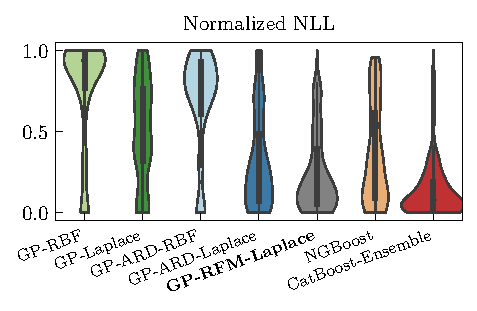
\includegraphics[trim=0 40 0 0, clip, width=\textwidth]{figures/tabularbenchmark_nll.pdf}
    \end{subfigure}
    \hfill
    \begin{subfigure}[b]{0.475\textwidth}  
        \centering 
        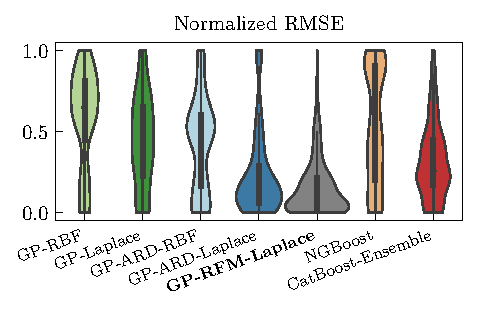
\includegraphics[trim=0 40 0 0, clip, width=\textwidth]{figures/tabularbenchmark_rmse.pdf}
    \end{subfigure}
    % \vskip\baselineskip
    \begin{subfigure}[b]{0.475\textwidth}   
        \centering 
        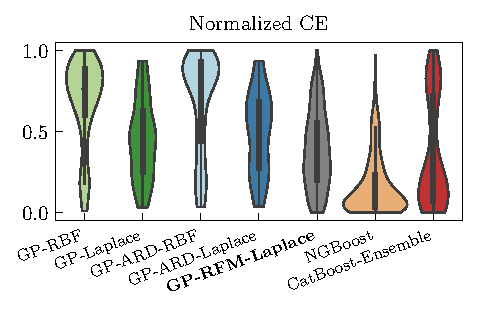
\includegraphics[width=\textwidth]{figures/tabularbenchmark_coverage.pdf}
    \end{subfigure}
    \hfill
    \begin{subfigure}[b]{0.475\textwidth}   
        \centering 
        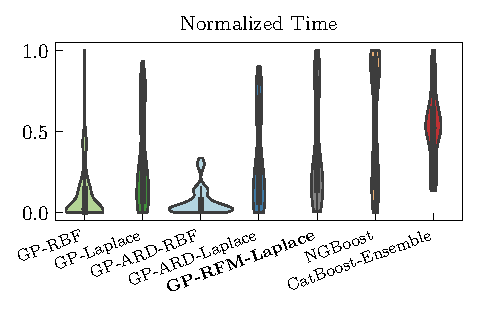
\includegraphics[width=\textwidth]{figures/tabularbenchmark_time.pdf}
    \end{subfigure}
    \caption{
        \hl{title TODO} results on tabular benchmark datasets
        \daniel{explanation: Every dataset of the 16 tabular benchmark dataset; tabular benchmark has more datasets/features/samples than uci benchmark we use; all hyperparameters are tuned; run everything for 20 seeds; for each dataset and metric we normalize the results of all methods in $[0,1]$; violin plot.}
        \daniel{use word 'coverage error'}
        } 
    \label{fig:main-tabular-benchmark-app}
\end{figure*}

\begin{figure*}[htb]
    \centering
    \begin{subfigure}[b]{0.475\textwidth}
        \centering
        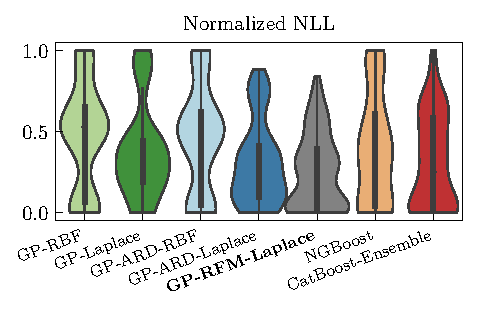
\includegraphics[trim=0 40 0 0, clip, width=\textwidth]{figures/uci_nll.pdf}
    \end{subfigure}
    \hfill
    \begin{subfigure}[b]{0.475\textwidth}  
        \centering 
        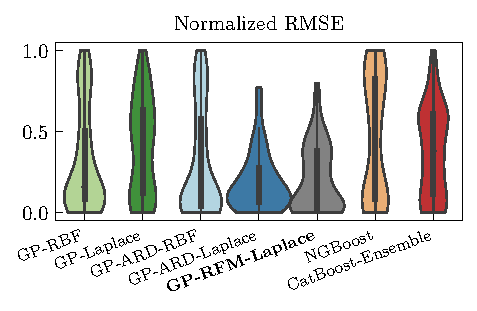
\includegraphics[trim=0 40 0 0, clip, width=\textwidth]{figures/uci_rmse.pdf}
    \end{subfigure}
    % \vskip\baselineskip
    \begin{subfigure}[b]{0.475\textwidth}   
        \centering 
        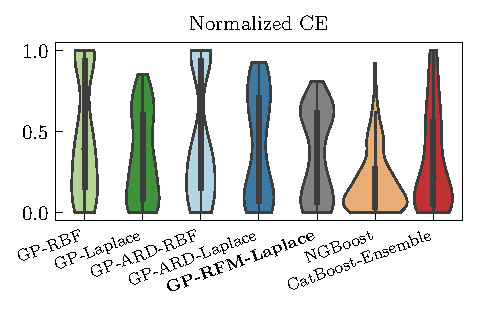
\includegraphics[width=\textwidth]{figures/uci_coverage.pdf}
    \end{subfigure}
    \hfill
    \begin{subfigure}[b]{0.475\textwidth}   
        \centering 
        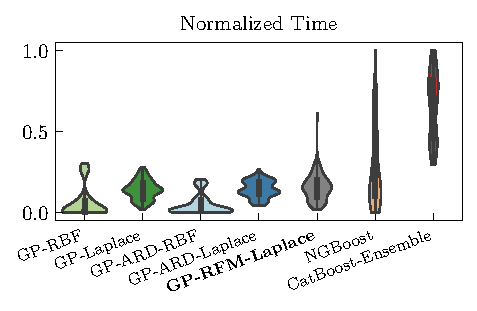
\includegraphics[width=\textwidth]{figures/uci_time.pdf}
    \end{subfigure}
    \caption{
        \hl{title TODO} results on UCI datasets. Complementary to \Cref{fig:main-tabular-benchmark}.
        \daniel{explanation: same as in \Cref{fig:main-tabular-benchmark}}
        } 
    \label{fig:main-uci}
\end{figure*}



\subsection{Comparative feature evaluation}



\begin{figure*}[htb]
    \centering
    \begin{subfigure}[b]{0.475\textwidth}
        \centering
        % \includegraphics{figuresTikz/feature_importance_nll}
        % \tikzsetnextfilename{feature_importance_nll}
        \begin{tikzpicture}[baseline]

\pgfplotstableread[col sep=comma]{./data/feature_importance_metrics.csv}{\datatable};
\begin{axis}[
width=\columnwidth,
height=.7\columnwidth,
ylabel={NLL},
xlabel={Fraction of remaining features},
title={Performance when removing features},
% ymax=0.3,
legend style={font=\tiny, 
	fill opacity=0.6, text opacity =1,
        at={(0.02, 0.02)},anchor=south west,
        row sep=-3pt,
        },
legend cell align={left},
% ytick={0, 0.08}, % Define the desired y tick positions
xtick={60, 70, 80, 90, 100}, % Define the desired y tick positions
xticklabels={60\%, 70\%, 80\%, 90\%, 100\%},
yticklabel style={
	% /pgf/number format/fixed, % Use fixed point notation
	% /pgf/number format/precision=2, % Set the number of decimal places
	% /pgf/number format/fixed zerofill, % Fill in trailing zeros
        },
% ymode=log,
]

% GP-RBF
\addplot+ [lightgreen, mark=*, 
mark options={solid},
thick,
% error bars/.cd,
% x dir=both,x explicit,
% y dir=both,y explicit,
% error bar style={solid}
]
table[x=features,y=GP_RBF_NLPD_mean,y error=GP_RBF_NLPD_std] {\datatable};


% GP-Laplace
\addplot+ [darkgreen, mark=*, 
mark options={solid},
thick,
% error bars/.cd,
% x dir=both,x explicit,
% y dir=both,y explicit,
% error bar style={solid}
]
table[x=features,y=GP_Laplace_NLPD_mean,y error=GP_Laplace_NLPD_std] {\datatable};


% GP-ARD-RBF
\addplot+ [lightblue, mark=*, 
mark options={solid},
thick,
dotted,
% error bars/.cd,
% x dir=both,x explicit,
% y dir=both,y explicit,
% error bar style={solid}
]
table[x=features,y=GP_ARD_RBF_NLPD_mean,y error=GP_ARD_RBF_NLPD_std] {\datatable};


% GP-ARD-Laplace
\addplot+ [darkblue, mark=*, 
mark options={solid},
thick,
dotted,
% error bars/.cd,
% x dir=both,x explicit,
% y dir=both,y explicit,
% error bar style={solid}
]
table[x=features,y=GP_ARD_Laplace_NLPD_mean,y error=GP_ARD_Laplace_NLPD_std] {\datatable};


% RFM
\addplot+ [black, mark=*, 
mark options={solid},
thick,
% error bars/.cd,
% x dir=both,x explicit,
% y dir=both,y explicit,
% error bar style={solid}
]
table[x=features,y=GP_RFM_Laplace_NLPD_mean,y error=GP_RFM_Laplace_NLPD_std] {\datatable};


% NG-Boost
\addplot+ [orange, mark=*, 
mark options={solid},
thick,
dashed,
% error bars/.cd,
% x dir=both,x explicit,
% y dir=both,y explicit,
% error bar style={solid}
]
table[x=features,y=NG_Boost_NLPD_mean,y error=GP_RFM_Laplace_NLPD_std] {\datatable};


% Cat-Boost-Ensemble
\addplot+ [red, mark=*, 
mark options={solid},
thick,
dashed,
% error bars/.cd,
% x dir=both,x explicit,
% y dir=both,y explicit,
% error bar style={solid}
]
table[x=features,y=Cat_Boost_Ensemble_NLPD_mean,y error=Cat_Boost_Ensemble_NLPD_std] {\datatable};



\legend{
    {GP-RBF},
    {GP-Laplace},
    {GP-ARD-RBF},
    {GP-ARD-Laplace},
    {GP-RFM-Laplace}, 
    {NGBoost},
    {CatBoost-Ensemble}
}

\end{axis}
\end{tikzpicture}
    \end{subfigure}
    \hfill
    \begin{subfigure}[b]{0.475\textwidth}  
        \centering
        % \includegraphics{figuresTikz/feature_importance_rmse}
        % \tikzsetnextfilename{feature_importance_rmse}
        \begin{tikzpicture}[baseline]

\pgfplotstableread[col sep=comma]{./data/feature_importance_metrics.csv}{\datatable};
\begin{axis}[
width=1\columnwidth,
height=.7\columnwidth,
ylabel={RMSE},
xlabel={Fraction of remaining features},
title={Performance when removing features},
% ymax=0.3,
legend style={font=\tiny, 
	fill opacity=0.6, text opacity =1,
        at={(0.02, 0.02)},anchor=south west,
        row sep=-3pt,
        },
legend cell align={left},
% ytick={0, 0.08}, % Define the desired y tick positions
xtick={60, 70, 80, 90, 100}, % Define the desired y tick positions
xticklabels={60\%, 70\%, 80\%, 90\%, 100\%},
yticklabel style={
	% /pgf/number format/fixed, % Use fixed point notation
	% /pgf/number format/precision=2, % Set the number of decimal places
	% /pgf/number format/fixed zerofill, % Fill in trailing zeros
        },
% ymode=log,
]

% GP-RBF
\addplot+ [lightgreen, mark=*, 
mark options={solid},
thick,
% error bars/.cd,
% x dir=both,x explicit,
% y dir=both,y explicit,
% error bar style={solid}
]
table[x=features,y=GP_RBF_RMSE_mean,y error=GP_RBF_RMSE_std] {\datatable};


% GP-Laplace
\addplot+ [darkgreen, mark=*, 
mark options={solid},
thick,
% error bars/.cd,
% x dir=both,x explicit,
% y dir=both,y explicit,
% error bar style={solid}
]
table[x=features,y=GP_Laplace_RMSE_mean,y error=GP_Laplace_RMSE_std] {\datatable};


% GP-ARD-RBF
\addplot+ [lightblue, mark=*, 
mark options={solid},
thick,
dotted,
% error bars/.cd,
% x dir=both,x explicit,
% y dir=both,y explicit,
% error bar style={solid}
]
table[x=features,y=GP_ARD_RBF_RMSE_mean,y error=GP_ARD_RBF_RMSE_std] {\datatable};


% GP-ARD-Laplace
\addplot+ [darkblue, mark=*, 
mark options={solid},
thick,
dotted,
% error bars/.cd,
% x dir=both,x explicit,
% y dir=both,y explicit,
% error bar style={solid}
]
table[x=features,y=GP_ARD_Laplace_RMSE_mean,y error=GP_ARD_Laplace_RMSE_std] {\datatable};


% RFM
\addplot+ [black, mark=*, 
mark options={solid},
thick,
% error bars/.cd,
% x dir=both,x explicit,
% y dir=both,y explicit,
% error bar style={solid}
]
table[x=features,y=GP_RFM_Laplace_RMSE_mean,y error=GP_RFM_Laplace_RMSE_std] {\datatable};


% NG-Boost
\addplot+ [orange, mark=*, 
mark options={solid},
thick,
dashed,
% error bars/.cd,
% x dir=both,x explicit,
% y dir=both,y explicit,
% error bar style={solid}
]
table[x=features,y=NG_Boost_RMSE_mean,y error=GP_RFM_Laplace_RMSE_std] {\datatable};


% Cat-Boost-Ensemble
\addplot+ [red, mark=*, 
mark options={solid},
thick,
dashed,
% error bars/.cd,
% x dir=both,x explicit,
% y dir=both,y explicit,
% error bar style={solid}
]
table[x=features,y=Cat_Boost_Ensemble_RMSE_mean,y error=Cat_Boost_Ensemble_RMSE_std] {\datatable};



\legend{
    {GP-RBF},
    {GP-Laplace},
    {GP-ARD-RBF},
    {GP-ARD-Laplace},
    {GP-RFM-Laplace}, 
    {NGBoost},
    {CatBoost Ensemble}
}

\end{axis}
\end{tikzpicture}
    \end{subfigure}
    \caption{NLL (left) and RMSE (right) when removing the most important features according to the diagonal of the RFM weight matrix.} 
    \label{fig:feature-importance}
\end{figure*}
    







\subsection{Toy data set}

\begin{figure}[htb]
    \centering
    % \includegraphics{figuresTikz/toy_data_rmse}
    % \tikzsetnextfilename{toy_data_rmse}
    \begin{tikzpicture}[baseline]

\pgfplotstableread[col sep=comma]{./data/toy_data_metrics.csv}{\datatable};
\begin{axis}[
width=0.5\columnwidth,
height=.35\columnwidth,
ylabel={RMSE},
xlabel={features},
title={Toy data with feature correlation},
xmin=19,
xmax=131,
% ymin=0,
% ymax=0.33,
legend style={font=\tiny, 
	fill opacity=0.6, text opacity =1,
        % at={(1.,1)},anchor=north east,
        row sep=-3pt,
        },
legend cell align={left},
% ytick={0, 0.08}, % Define the desired y tick positions
xtick={10, 30, 50, 70, 90, 110, 130}, % Define the desired y tick positions
yticklabel style={
	% /pgf/number format/fixed, % Use fixed point notation
	% /pgf/number format/precision=2, % Set the number of decimal places
	% /pgf/number format/fixed zerofill, % Fill in trailing zeros
        },
% ymode=log,
]


% RFM full
\addplot+ [black, 
mark=*, 
mark options={solid},
% mark size=5pt, 
thick,
error bars/.cd,
x dir=both,x explicit,
y dir=both,y explicit,
error bar style={solid}
]
table[x=features,y=GP_RFM_Laplace_full_RMSE_mean,y error=GP_RFM_Laplace_full_RMSE_std] {\datatable};

% % RFM diag
% \addplot+ [red, mark=x, mark size=5pt, thick,
% error bars/.cd,
% x dir=both,x explicit,
% y dir=both,y explicit,
% error bar style={solid}
% ]
% table[x=features,y=GP_RFM_Laplace_diag_RMSE_mean,y error=GP_RFM_Laplace_diag_RMSE_std] {\datatable};

% Laplace
\addplot+ [darkgreen, 
mark=*, 
mark options={solid},
% mark size=5pt, 
thick,
error bars/.cd,
x dir=both,x explicit,
y dir=both,y explicit,
error bar style={solid}
]
table[x=features,y=GP_Laplace_RMSE_mean,y error=GP_Laplace_RMSE_std] {\datatable};

% ARD-Laplace
\addplot+ [darkblue, 
dotted,
mark=*, 
mark options={solid},
% mark size=5pt, 
thick,
error bars/.cd,
x dir=both,x explicit,
y dir=both,y explicit,
error bar style={solid}
]
table[x=features,y=GP_ARD_Laplace_RMSE_mean,y error=GP_ARD_Laplace_RMSE_std] {\datatable};

% NG-boost
\addplot+ [orange, 
dashed,
mark=*, 
mark options={solid},
% mark size=5pt, 
thick,
error bars/.cd,
x dir=both,x explicit,
y dir=both,y explicit,
error bar style={solid}
]
table[x=features,y=NG_Boost_RMSE_mean,y error=NG_Boost_RMSE_std] {\datatable};

% Cat-Boost Ensemble
\addplot+ [red, 
dashed,
mark=*, 
mark options={solid},
% mark size=5pt, 
thick,
error bars/.cd,
x dir=both,x explicit,
y dir=both,y explicit,
error bar style={solid}
]
table[x=features,y=Cat_Boost_Ensemble_RMSE_mean,y error=Cat_Boost_Ensemble_RMSE_std] {\datatable};



\legend{
    {GP-RFM}, 
    {GP-Laplace},
    % {GP-RFM-diag},
    {GP-ARD-Laplace},
    {NGBoost},
    {CatBoost Ensemble}
}

\end{axis}
\end{tikzpicture}
    \caption{
        \hl{Title TODO} Complementary to \Cref{fig:toy-data-nll} but showing RMSE instead of NLL here.
        \daniel{Explanation: Same as in \Cref{fig:toy-data-nll}.}
        }
    \label{fig:toy-data-rmse}
\end{figure}

\hl{Include figure about learnt feature matrix in RFM, RFM-diag and ARD-Laplace as comprison}








\subsection{Distribution shift}


\begin{figure*}[htb]
    \centering
    \begin{subfigure}[b]{0.475\textwidth}
        \centering
        % \includegraphics{figuresTikz/ood_covariate_nll}
        % \tikzsetnextfilename{ood_covariate_nll}
        \begin{tikzpicture}[baseline]

\pgfplotstableread[col sep=comma]{./data/ood_covariate_metrics.csv}{\datatable};
\begin{axis}[
width=\columnwidth,
height=.7\columnwidth,
% ylabel={NLL},
% xlabel={},
title={NLL},
ymax=2,
legend style={font=\tiny, 
	fill opacity=0.6, text opacity =1,
        at={(0.02, 0.98)},anchor=north west,
        row sep=-3pt,
        },
legend cell align={left},
% ytick={0, 0.08}, % Define the desired y tick positions
xtick={0, 1,2,3,4}, % Define the desired y tick positions
xticklabels={ID, OOD-1, OOD-2, OOD-3, OOD-4},
yticklabel style={
	% /pgf/number format/fixed, % Use fixed point notation
	% /pgf/number format/precision=2, % Set the number of decimal places
	% /pgf/number format/fixed zerofill, % Fill in trailing zeros
        },
% ymode=log,
]

% GP-RBF
\addplot+ [lightgreen, mark=*, 
mark options={solid},
thick,
% error bars/.cd,
% x dir=both,x explicit,
% y dir=both,y explicit,
% error bar style={solid}
]
table[x=test_level,y=GP_RBF_NLPD_mean,y error=GP_RBF_NLPD_std] {\datatable};


% GP-Laplace
\addplot+ [darkgreen, mark=*, 
mark options={solid},
thick,
% error bars/.cd,
% x dir=both,x explicit,
% y dir=both,y explicit,
% error bar style={solid}
]
table[x=test_level,y=GP_Laplace_NLPD_mean,y error=GP_Laplace_NLPD_std] {\datatable};


% GP-ARD-RBF
\addplot+ [lightblue, mark=*, 
mark options={solid},
thick,
dotted,
% error bars/.cd,
% x dir=both,x explicit,
% y dir=both,y explicit,
% error bar style={solid}
]
table[x=test_level,y=GP_ARD_RBF_NLPD_mean,y error=GP_ARD_RBF_NLPD_std] {\datatable};


% GP-ARD-Laplace
\addplot+ [darkblue, mark=*, 
mark options={solid},
thick,
dotted,
% error bars/.cd,
% x dir=both,x explicit,
% y dir=both,y explicit,
% error bar style={solid}
]
table[x=test_level,y=GP_ARD_Laplace_NLPD_mean,y error=GP_ARD_Laplace_NLPD_std] {\datatable};


% RFM
\addplot+ [black, mark=*, 
mark options={solid},
thick,
% error bars/.cd,
% x dir=both,x explicit,
% y dir=both,y explicit,
% error bar style={solid}
]
table[x=test_level,y=GP_RFM_Laplace_NLPD_mean,y error=GP_RFM_Laplace_NLPD_std] {\datatable};


% NG-Boost
\addplot+ [orange, mark=*, 
mark options={solid},
thick,
dashed,
% error bars/.cd,
% x dir=both,x explicit,
% y dir=both,y explicit,
% error bar style={solid}
]
table[x=test_level,y=NG_Boost_NLPD_mean,y error=GP_RFM_Laplace_NLPD_std] {\datatable};


% Cat-Boost-Ensemble
\addplot+ [red, mark=*, 
mark options={solid},
thick,
dashed,
% error bars/.cd,
% x dir=both,x explicit,
% y dir=both,y explicit,
% error bar style={solid}
]
table[x=test_level,y=Cat_Boost_Ensemble_NLPD_mean,y error=Cat_Boost_Ensemble_NLPD_std] {\datatable};



% \legend{
%     {GP-RBF},
%     {GP-Laplace},
%     {GP-ARD-RBF},
%     {GP-ARD-Laplace},
%     {GP-RFM-Laplace}, 
%     {NGBoost},
%     {CatBoost-Ensemble}
% }

\end{axis}
\end{tikzpicture}
    \end{subfigure}
    \hfill
    \begin{subfigure}[b]{0.475\textwidth}  
        \centering
        % \includegraphics{figuresTikz/ood_covariate_rmse}
        % \tikzsetnextfilename{ood_covariate_rmse}
        \begin{tikzpicture}[baseline]

\pgfplotstableread[col sep=comma]{./data/ood_covariate_metrics.csv}{\datatable};
\begin{axis}[
width=\columnwidth,
height=.7\columnwidth,
% ylabel={RMSE},
% xlabel={},
title={RMSE},
% ymax=2,
legend style={font=\tiny, 
	fill opacity=0.6, text opacity =1,
        at={(0.02, 0.98)},anchor=north west,
        row sep=-3pt,
        },
legend cell align={left},
% ytick={0, 0.08}, % Define the desired y tick positions
xtick={0, 1,2,3,4}, % Define the desired y tick positions
xticklabels={ID, OOD-1, OOD-2, OOD-3, OOD-4},
yticklabel style={
	% /pgf/number format/fixed, % Use fixed point notation
	% /pgf/number format/precision=2, % Set the number of decimal places
	% /pgf/number format/fixed zerofill, % Fill in trailing zeros
        },
% ymode=log,
]

% GP-RBF
\addplot+ [lightgreen, mark=*, 
mark options={solid},
thick,
% error bars/.cd,
% x dir=both,x explicit,
% y dir=both,y explicit,
% error bar style={solid}
]
table[x=test_level,y=GP_RBF_RMSE_mean,y error=GP_RBF_RMSE_std] {\datatable};


% GP-Laplace
\addplot+ [darkgreen, mark=*, 
mark options={solid},
thick,
% error bars/.cd,
% x dir=both,x explicit,
% y dir=both,y explicit,
% error bar style={solid}
]
table[x=test_level,y=GP_Laplace_RMSE_mean,y error=GP_Laplace_RMSE_std] {\datatable};


% GP-ARD-RBF
\addplot+ [lightblue, mark=*, 
mark options={solid},
thick,
dotted,
% error bars/.cd,
% x dir=both,x explicit,
% y dir=both,y explicit,
% error bar style={solid}
]
table[x=test_level,y=GP_ARD_RBF_RMSE_mean,y error=GP_ARD_RBF_RMSE_std] {\datatable};


% GP-ARD-Laplace
\addplot+ [darkblue, mark=*, 
mark options={solid},
thick,
dotted,
% error bars/.cd,
% x dir=both,x explicit,
% y dir=both,y explicit,
% error bar style={solid}
]
table[x=test_level,y=GP_ARD_Laplace_RMSE_mean,y error=GP_ARD_Laplace_RMSE_std] {\datatable};


% RFM
\addplot+ [black, mark=*, 
mark options={solid},
thick,
% error bars/.cd,
% x dir=both,x explicit,
% y dir=both,y explicit,
% error bar style={solid}
]
table[x=test_level,y=GP_RFM_Laplace_RMSE_mean,y error=GP_RFM_Laplace_RMSE_std] {\datatable};


% NG-Boost
\addplot+ [orange, mark=*, 
mark options={solid},
thick,
dashed,
% error bars/.cd,
% x dir=both,x explicit,
% y dir=both,y explicit,
% error bar style={solid}
]
table[x=test_level,y=NG_Boost_RMSE_mean,y error=GP_RFM_Laplace_RMSE_std] {\datatable};


% Cat-Boost-Ensemble
\addplot+ [red, mark=*, 
mark options={solid},
thick,
dashed,
% error bars/.cd,
% x dir=both,x explicit,
% y dir=both,y explicit,
% error bar style={solid}
]
table[x=test_level,y=Cat_Boost_Ensemble_RMSE_mean,y error=Cat_Boost_Ensemble_RMSE_std] {\datatable};



\legend{
    {GP-RBF},
    {GP-Laplace},
    {GP-ARD-RBF},
    {GP-ARD-Laplace},
    {GP-RFM-Laplace}, 
    {NGBoost},
    {CatBoost-Ensemble}
}

\end{axis}
\end{tikzpicture}
    \end{subfigure}
    % \vskip\baselineskip
    \begin{subfigure}[b]{0.475\textwidth}   
        \centering
        % \includegraphics{figuresTikz/ood_covariate_coverage}
        % \tikzsetnextfilename{ood_covariate_coverage}
        \begin{tikzpicture}[baseline]

\pgfplotstableread[col sep=comma]{./data/ood_covariate_metrics.csv}{\datatable};
\begin{axis}[
width=\columnwidth,
height=.7\columnwidth,
% ylabel={Coverage},
% xlabel={},
title={Coverage Error},
% ymax=2,
legend style={font=\tiny, 
	fill opacity=0.6, text opacity =1,
        at={(0.02, 0.98)},anchor=north west,
        row sep=-3pt,
        },
legend cell align={left},
% ytick={0, 0.08}, % Define the desired y tick positions
xtick={0, 1,2,3,4}, % Define the desired y tick positions
xticklabels={ID, OOD-1, OOD-2, OOD-3, OOD-4},
yticklabel style={
	% /pgf/number format/fixed, % Use fixed point notation
	% /pgf/number format/precision=2, % Set the number of decimal places
	% /pgf/number format/fixed zerofill, % Fill in trailing zeros
        },
% ymode=log,
]

% GP-RBF
\addplot+ [lightgreen, mark=*, 
mark options={solid},
thick,
% error bars/.cd,
% x dir=both,x explicit,
% y dir=both,y explicit,
% error bar style={solid}
]
table[x=test_level,y=GP_RBF_Coverage_mean,y error=GP_RBF_Coverage_std] {\datatable};


% GP-Laplace
\addplot+ [darkgreen, mark=*, 
mark options={solid},
thick,
% error bars/.cd,
% x dir=both,x explicit,
% y dir=both,y explicit,
% error bar style={solid}
]
table[x=test_level,y=GP_Laplace_Coverage_mean,y error=GP_Laplace_Coverage_std] {\datatable};


% GP-ARD-RBF
\addplot+ [lightblue, mark=*, 
mark options={solid},
thick,
dotted,
% error bars/.cd,
% x dir=both,x explicit,
% y dir=both,y explicit,
% error bar style={solid}
]
table[x=test_level,y=GP_ARD_RBF_Coverage_mean,y error=GP_ARD_RBF_Coverage_std] {\datatable};


% GP-ARD-Laplace
\addplot+ [darkblue, mark=*, 
mark options={solid},
thick,
dotted,
% error bars/.cd,
% x dir=both,x explicit,
% y dir=both,y explicit,
% error bar style={solid}
]
table[x=test_level,y=GP_ARD_Laplace_Coverage_mean,y error=GP_ARD_Laplace_Coverage_std] {\datatable};


% RFM
\addplot+ [black, mark=*, 
mark options={solid},
thick,
% error bars/.cd,
% x dir=both,x explicit,
% y dir=both,y explicit,
% error bar style={solid}
]
table[x=test_level,y=GP_RFM_Laplace_Coverage_mean,y error=GP_RFM_Laplace_Coverage_std] {\datatable};


% NG-Boost
\addplot+ [orange, mark=*, 
mark options={solid},
thick,
dashed,
% error bars/.cd,
% x dir=both,x explicit,
% y dir=both,y explicit,
% error bar style={solid}
]
table[x=test_level,y=NG_Boost_Coverage_mean,y error=GP_RFM_Laplace_Coverage_std] {\datatable};


% Cat-Boost-Ensemble
\addplot+ [red, mark=*, 
mark options={solid},
thick,
dashed,
% error bars/.cd,
% x dir=both,x explicit,
% y dir=both,y explicit,
% error bar style={solid}
]
table[x=test_level,y=Cat_Boost_Ensemble_Coverage_mean,y error=Cat_Boost_Ensemble_Coverage_std] {\datatable};



% \legend{
%     {GP-RBF},
%     {GP-Laplace},
%     {GP-ARD-RBF},
%     {GP-ARD-Laplace},
%     {GP-RFM-Laplace}, 
%     {NGBoost},
%     {CatBoost-Ensemble}
% }

\end{axis}
\end{tikzpicture}
    \end{subfigure}     
    \hfill
    \begin{subfigure}[b]{0.475\textwidth}   
        \centering 
        % \includegraphics{figuresTikz/ood_covariate_intvallen}
        % \tikzsetnextfilename{ood_covariate_intvallen}
        \begin{tikzpicture}[baseline]

\pgfplotstableread[col sep=comma]{./data/ood_covariate_metrics.csv}{\datatable};
\begin{axis}[
width=\columnwidth,
height=.7\columnwidth,
% ylabel={Interval_Len},
% xlabel={},
title={Interval Length},
% ymax=2,
legend style={font=\tiny, 
	fill opacity=0.6, text opacity =1,
        at={(0.02, 0.98)},anchor=north west,
        row sep=-3pt,
        },
legend cell align={left},
% ytick={0, 0.08}, % Define the desired y tick positions
xtick={0, 1,2,3,4}, % Define the desired y tick positions
xticklabels={ID, OOD-1, OOD-2, OOD-3, OOD-4},
yticklabel style={
	% /pgf/number format/fixed, % Use fixed point notation
	% /pgf/number format/precision=2, % Set the number of decimal places
	% /pgf/number format/fixed zerofill, % Fill in trailing zeros
        },
% ymode=log,
]

% GP-RBF
\addplot+ [lightgreen, mark=*, 
mark options={solid},
thick,
% error bars/.cd,
% x dir=both,x explicit,
% y dir=both,y explicit,
% error bar style={solid}
]
table[x=test_level,y=GP_RBF_Interval_Len_mean,y error=GP_RBF_Interval_Len_std] {\datatable};


% GP-Laplace
\addplot+ [darkgreen, mark=*, 
mark options={solid},
thick,
% error bars/.cd,
% x dir=both,x explicit,
% y dir=both,y explicit,
% error bar style={solid}
]
table[x=test_level,y=GP_Laplace_Interval_Len_mean,y error=GP_Laplace_Interval_Len_std] {\datatable};


% GP-ARD-RBF
\addplot+ [lightblue, mark=*, 
mark options={solid},
thick,
dotted,
% error bars/.cd,
% x dir=both,x explicit,
% y dir=both,y explicit,
% error bar style={solid}
]
table[x=test_level,y=GP_ARD_RBF_Interval_Len_mean,y error=GP_ARD_RBF_Interval_Len_std] {\datatable};


% GP-ARD-Laplace
\addplot+ [darkblue, mark=*, 
mark options={solid},
thick,
dotted,
% error bars/.cd,
% x dir=both,x explicit,
% y dir=both,y explicit,
% error bar style={solid}
]
table[x=test_level,y=GP_ARD_Laplace_Interval_Len_mean,y error=GP_ARD_Laplace_Interval_Len_std] {\datatable};


% RFM
\addplot+ [black, mark=*, 
mark options={solid},
thick,
% error bars/.cd,
% x dir=both,x explicit,
% y dir=both,y explicit,
% error bar style={solid}
]
table[x=test_level,y=GP_RFM_Laplace_Interval_Len_mean,y error=GP_RFM_Laplace_Interval_Len_std] {\datatable};


% NG-Boost
\addplot+ [orange, mark=*, 
mark options={solid},
thick,
dashed,
% error bars/.cd,
% x dir=both,x explicit,
% y dir=both,y explicit,
% error bar style={solid}
]
table[x=test_level,y=NG_Boost_Interval_Len_mean,y error=GP_RFM_Laplace_Interval_Len_std] {\datatable};


% Cat-Boost-Ensemble
\addplot+ [red, mark=*, 
mark options={solid},
thick,
dashed,
% error bars/.cd,
% x dir=both,x explicit,
% y dir=both,y explicit,
% error bar style={solid}
]
table[x=test_level,y=Cat_Boost_Ensemble_Interval_Len_mean,y error=Cat_Boost_Ensemble_Interval_Len_std] {\datatable};



% \legend{
%     {GP-RBF},
%     {GP-Laplace},
%     {GP-ARD-RBF},
%     {GP-ARD-Laplace},
%     {GP-RFM-Laplace}, 
%     {NGBoost},
%     {CatBoost-Ensemble}
% }

\end{axis}
\end{tikzpicture}
    \end{subfigure}
    \caption{
        \hl{title TODO} Covariate shift......
        } 
    \label{fig:ood-covariate-appendix}
\end{figure*}


\begin{figure*}[htb]
    \centering
    \begin{subfigure}[b]{0.475\textwidth}
        \centering
        % \includegraphics{figuresTikz/ood_label_nll}
        % \tikzsetnextfilename{ood_label_nll}
        \begin{tikzpicture}[baseline]

\pgfplotstableread[col sep=comma]{./data/ood_label_metrics.csv}{\datatable};
\begin{axis}[
width=\columnwidth,
height=.7\columnwidth,
% ylabel={NLL},
% xlabel={},
title={NLL},
ymax=9,
legend style={font=\tiny, 
	fill opacity=0.6, text opacity =1,
        at={(0.02, 0.98)},anchor=north west,
        row sep=-3pt,
        },
legend cell align={left},
% ytick={0, 0.08}, % Define the desired y tick positions
xtick={0, 1,2,3,4}, % Define the desired y tick positions
xticklabels={ID, OOD-1, OOD-2, OOD-3, OOD-4},
yticklabel style={
	% /pgf/number format/fixed, % Use fixed point notation
	% /pgf/number format/precision=2, % Set the number of decimal places
	% /pgf/number format/fixed zerofill, % Fill in trailing zeros
        },
% ymode=log,
]

% GP-RBF
\addplot+ [lightgreen, mark=*, 
mark options={solid},
thick,
% error bars/.cd,
% x dir=both,x explicit,
% y dir=both,y explicit,
% error bar style={solid}
]
table[x=test_level,y=GP_RBF_NLPD_mean,y error=GP_RBF_NLPD_std] {\datatable};


% GP-Laplace
\addplot+ [darkgreen, mark=*, 
mark options={solid},
thick,
% error bars/.cd,
% x dir=both,x explicit,
% y dir=both,y explicit,
% error bar style={solid}
]
table[x=test_level,y=GP_Laplace_NLPD_mean,y error=GP_Laplace_NLPD_std] {\datatable};


% GP-ARD-RBF
\addplot+ [lightblue, mark=*, 
mark options={solid},
thick,
dotted,
% error bars/.cd,
% x dir=both,x explicit,
% y dir=both,y explicit,
% error bar style={solid}
]
table[x=test_level,y=GP_ARD_RBF_NLPD_mean,y error=GP_ARD_RBF_NLPD_std] {\datatable};


% GP-ARD-Laplace
\addplot+ [darkblue, mark=*, 
mark options={solid},
thick,
dotted,
% error bars/.cd,
% x dir=both,x explicit,
% y dir=both,y explicit,
% error bar style={solid}
]
table[x=test_level,y=GP_ARD_Laplace_NLPD_mean,y error=GP_ARD_Laplace_NLPD_std] {\datatable};


% RFM
\addplot+ [black, mark=*, 
mark options={solid},
thick,
% error bars/.cd,
% x dir=both,x explicit,
% y dir=both,y explicit,
% error bar style={solid}
]
table[x=test_level,y=GP_RFM_Laplace_NLPD_mean,y error=GP_RFM_Laplace_NLPD_std] {\datatable};


% NG-Boost
\addplot+ [orange, mark=*, 
mark options={solid},
thick,
dashed,
% error bars/.cd,
% x dir=both,x explicit,
% y dir=both,y explicit,
% error bar style={solid}
]
table[x=test_level,y=NG_Boost_NLPD_mean,y error=GP_RFM_Laplace_NLPD_std] {\datatable};


% Cat-Boost-Ensemble
\addplot+ [red, mark=*, 
mark options={solid},
thick,
dashed,
% error bars/.cd,
% x dir=both,x explicit,
% y dir=both,y explicit,
% error bar style={solid}
]
table[x=test_level,y=Cat_Boost_Ensemble_NLPD_mean,y error=Cat_Boost_Ensemble_NLPD_std] {\datatable};



% \legend{
%     {GP-RBF},
%     {GP-Laplace},
%     {GP-ARD-RBF},
%     {GP-ARD-Laplace},
%     {GP-RFM-Laplace}, 
%     {NGBoost},
%     {CatBoost-Ensemble}
% }

\end{axis}
\end{tikzpicture}
    \end{subfigure}
    \hfill
    \begin{subfigure}[b]{0.475\textwidth}  
        \centering
        % \includegraphics{figuresTikz/ood_label_rmse}
        % \tikzsetnextfilename{ood_label_rmse}
        \begin{tikzpicture}[baseline]

\pgfplotstableread[col sep=comma]{./data/ood_label_metrics.csv}{\datatable};
\begin{axis}[
width=\columnwidth,
height=.7\columnwidth,
% ylabel={RMSE},
% xlabel={},
title={RMSE},
% ymax=2,
legend style={font=\tiny, 
	fill opacity=0.6, text opacity =1,
        at={(0.02, 0.98)},anchor=north west,
        row sep=-3pt,
        },
legend cell align={left},
% ytick={0, 0.08}, % Define the desired y tick positions
xtick={0, 1,2,3,4}, % Define the desired y tick positions
xticklabels={ID, OOD-1, OOD-2, OOD-3, OOD-4},
yticklabel style={
	% /pgf/number format/fixed, % Use fixed point notation
	% /pgf/number format/precision=2, % Set the number of decimal places
	% /pgf/number format/fixed zerofill, % Fill in trailing zeros
        },
% ymode=log,
]

% GP-RBF
\addplot+ [lightgreen, mark=*, 
mark options={solid},
thick,
% error bars/.cd,
% x dir=both,x explicit,
% y dir=both,y explicit,
% error bar style={solid}
]
table[x=test_level,y=GP_RBF_RMSE_mean,y error=GP_RBF_RMSE_std] {\datatable};


% GP-Laplace
\addplot+ [darkgreen, mark=*, 
mark options={solid},
thick,
% error bars/.cd,
% x dir=both,x explicit,
% y dir=both,y explicit,
% error bar style={solid}
]
table[x=test_level,y=GP_Laplace_RMSE_mean,y error=GP_Laplace_RMSE_std] {\datatable};


% GP-ARD-RBF
\addplot+ [lightblue, mark=*, 
mark options={solid},
thick,
dotted,
% error bars/.cd,
% x dir=both,x explicit,
% y dir=both,y explicit,
% error bar style={solid}
]
table[x=test_level,y=GP_ARD_RBF_RMSE_mean,y error=GP_ARD_RBF_RMSE_std] {\datatable};


% GP-ARD-Laplace
\addplot+ [darkblue, mark=*, 
mark options={solid},
thick,
dotted,
% error bars/.cd,
% x dir=both,x explicit,
% y dir=both,y explicit,
% error bar style={solid}
]
table[x=test_level,y=GP_ARD_Laplace_RMSE_mean,y error=GP_ARD_Laplace_RMSE_std] {\datatable};


% RFM
\addplot+ [black, mark=*, 
mark options={solid},
thick,
% error bars/.cd,
% x dir=both,x explicit,
% y dir=both,y explicit,
% error bar style={solid}
]
table[x=test_level,y=GP_RFM_Laplace_RMSE_mean,y error=GP_RFM_Laplace_RMSE_std] {\datatable};


% NG-Boost
\addplot+ [orange, mark=*, 
mark options={solid},
thick,
dashed,
% error bars/.cd,
% x dir=both,x explicit,
% y dir=both,y explicit,
% error bar style={solid}
]
table[x=test_level,y=NG_Boost_RMSE_mean,y error=GP_RFM_Laplace_RMSE_std] {\datatable};


% Cat-Boost-Ensemble
\addplot+ [red, mark=*, 
mark options={solid},
thick,
dashed,
% error bars/.cd,
% x dir=both,x explicit,
% y dir=both,y explicit,
% error bar style={solid}
]
table[x=test_level,y=Cat_Boost_Ensemble_RMSE_mean,y error=Cat_Boost_Ensemble_RMSE_std] {\datatable};



\legend{
    {GP-RBF},
    {GP-Laplace},
    {GP-ARD-RBF},
    {GP-ARD-Laplace},
    {GP-RFM-Laplace}, 
    {NGBoost},
    {CatBoost-Ensemble}
}

\end{axis}
\end{tikzpicture}
    \end{subfigure}
    % \vskip\baselineskip
    \begin{subfigure}[b]{0.475\textwidth}   
        \centering
        % \includegraphics{figuresTikz/ood_label_coverage}
        % \tikzsetnextfilename{ood_label_coverage}
        \begin{tikzpicture}[baseline]

\pgfplotstableread[col sep=comma]{./data/ood_label_metrics.csv}{\datatable};
\begin{axis}[
width=\columnwidth,
height=.7\columnwidth,
% ylabel={Coverage},
% xlabel={},
title={Coverage Error},
% ymax=2,
legend style={font=\tiny, 
	fill opacity=0.6, text opacity =1,
        at={(0.02, 0.98)},anchor=north west,
        row sep=-3pt,
        },
legend cell align={left},
% ytick={0, 0.08}, % Define the desired y tick positions
xtick={0, 1,2,3,4}, % Define the desired y tick positions
xticklabels={ID, OOD-1, OOD-2, OOD-3, OOD-4},
yticklabel style={
	% /pgf/number format/fixed, % Use fixed point notation
	% /pgf/number format/precision=2, % Set the number of decimal places
	% /pgf/number format/fixed zerofill, % Fill in trailing zeros
        },
% ymode=log,
]

% GP-RBF
\addplot+ [lightgreen, mark=*, 
mark options={solid},
thick,
% error bars/.cd,
% x dir=both,x explicit,
% y dir=both,y explicit,
% error bar style={solid}
]
table[x=test_level,y=GP_RBF_Coverage_mean,y error=GP_RBF_Coverage_std] {\datatable};


% GP-Laplace
\addplot+ [darkgreen, mark=*, 
mark options={solid},
thick,
% error bars/.cd,
% x dir=both,x explicit,
% y dir=both,y explicit,
% error bar style={solid}
]
table[x=test_level,y=GP_Laplace_Coverage_mean,y error=GP_Laplace_Coverage_std] {\datatable};


% GP-ARD-RBF
\addplot+ [lightblue, mark=*, 
mark options={solid},
thick,
dotted,
% error bars/.cd,
% x dir=both,x explicit,
% y dir=both,y explicit,
% error bar style={solid}
]
table[x=test_level,y=GP_ARD_RBF_Coverage_mean,y error=GP_ARD_RBF_Coverage_std] {\datatable};


% GP-ARD-Laplace
\addplot+ [darkblue, mark=*, 
mark options={solid},
thick,
dotted,
% error bars/.cd,
% x dir=both,x explicit,
% y dir=both,y explicit,
% error bar style={solid}
]
table[x=test_level,y=GP_ARD_Laplace_Coverage_mean,y error=GP_ARD_Laplace_Coverage_std] {\datatable};


% RFM
\addplot+ [black, mark=*, 
mark options={solid},
thick,
% error bars/.cd,
% x dir=both,x explicit,
% y dir=both,y explicit,
% error bar style={solid}
]
table[x=test_level,y=GP_RFM_Laplace_Coverage_mean,y error=GP_RFM_Laplace_Coverage_std] {\datatable};


% NG-Boost
\addplot+ [orange, mark=*, 
mark options={solid},
thick,
dashed,
% error bars/.cd,
% x dir=both,x explicit,
% y dir=both,y explicit,
% error bar style={solid}
]
table[x=test_level,y=NG_Boost_Coverage_mean,y error=GP_RFM_Laplace_Coverage_std] {\datatable};


% Cat-Boost-Ensemble
\addplot+ [red, mark=*, 
mark options={solid},
thick,
dashed,
% error bars/.cd,
% x dir=both,x explicit,
% y dir=both,y explicit,
% error bar style={solid}
]
table[x=test_level,y=Cat_Boost_Ensemble_Coverage_mean,y error=Cat_Boost_Ensemble_Coverage_std] {\datatable};



% \legend{
%     {GP-RBF},
%     {GP-Laplace},
%     {GP-ARD-RBF},
%     {GP-ARD-Laplace},
%     {GP-RFM-Laplace}, 
%     {NGBoost},
%     {CatBoost-Ensemble}
% }

\end{axis}
\end{tikzpicture}
    \end{subfigure}
    \hfill
    \begin{subfigure}[b]{0.475\textwidth}   
        \centering 
        % \includegraphics{figuresTikz/ood_label_intvallen}
        % \tikzsetnextfilename{ood_label_intvallen}
        \begin{tikzpicture}[baseline]

\pgfplotstableread[col sep=comma]{./data/ood_label_metrics.csv}{\datatable};
\begin{axis}[
width=\columnwidth,
height=.7\columnwidth,
% ylabel={Interval_Len},
% xlabel={},
title={Interval Length},
% ymax=2,
legend style={font=\tiny, 
	fill opacity=0.6, text opacity =1,
        at={(0.02, 0.98)},anchor=north west,
        row sep=-3pt,
        },
legend cell align={left},
% ytick={0, 0.08}, % Define the desired y tick positions
xtick={0, 1,2,3,4}, % Define the desired y tick positions
xticklabels={ID, OOD-1, OOD-2, OOD-3, OOD-4},
yticklabel style={
	% /pgf/number format/fixed, % Use fixed point notation
	% /pgf/number format/precision=2, % Set the number of decimal places
	% /pgf/number format/fixed zerofill, % Fill in trailing zeros
        },
% ymode=log,
]

% GP-RBF
\addplot+ [lightgreen, mark=*, 
mark options={solid},
thick,
% error bars/.cd,
% x dir=both,x explicit,
% y dir=both,y explicit,
% error bar style={solid}
]
table[x=test_level,y=GP_RBF_Interval_Len_mean,y error=GP_RBF_Interval_Len_std] {\datatable};


% GP-Laplace
\addplot+ [darkgreen, mark=*, 
mark options={solid},
thick,
% error bars/.cd,
% x dir=both,x explicit,
% y dir=both,y explicit,
% error bar style={solid}
]
table[x=test_level,y=GP_Laplace_Interval_Len_mean,y error=GP_Laplace_Interval_Len_std] {\datatable};


% GP-ARD-RBF
\addplot+ [lightblue, mark=*, 
mark options={solid},
thick,
dotted,
% error bars/.cd,
% x dir=both,x explicit,
% y dir=both,y explicit,
% error bar style={solid}
]
table[x=test_level,y=GP_ARD_RBF_Interval_Len_mean,y error=GP_ARD_RBF_Interval_Len_std] {\datatable};


% GP-ARD-Laplace
\addplot+ [darkblue, mark=*, 
mark options={solid},
thick,
dotted,
% error bars/.cd,
% x dir=both,x explicit,
% y dir=both,y explicit,
% error bar style={solid}
]
table[x=test_level,y=GP_ARD_Laplace_Interval_Len_mean,y error=GP_ARD_Laplace_Interval_Len_std] {\datatable};


% RFM
\addplot+ [black, mark=*, 
mark options={solid},
thick,
% error bars/.cd,
% x dir=both,x explicit,
% y dir=both,y explicit,
% error bar style={solid}
]
table[x=test_level,y=GP_RFM_Laplace_Interval_Len_mean,y error=GP_RFM_Laplace_Interval_Len_std] {\datatable};


% NG-Boost
\addplot+ [orange, mark=*, 
mark options={solid},
thick,
dashed,
% error bars/.cd,
% x dir=both,x explicit,
% y dir=both,y explicit,
% error bar style={solid}
]
table[x=test_level,y=NG_Boost_Interval_Len_mean,y error=GP_RFM_Laplace_Interval_Len_std] {\datatable};


% Cat-Boost-Ensemble
\addplot+ [red, mark=*, 
mark options={solid},
thick,
dashed,
% error bars/.cd,
% x dir=both,x explicit,
% y dir=both,y explicit,
% error bar style={solid}
]
table[x=test_level,y=Cat_Boost_Ensemble_Interval_Len_mean,y error=Cat_Boost_Ensemble_Interval_Len_std] {\datatable};



% \legend{
%     {GP-RBF},
%     {GP-Laplace},
%     {GP-ARD-RBF},
%     {GP-ARD-Laplace},
%     {GP-RFM-Laplace}, 
%     {NGBoost},
%     {CatBoost-Ensemble}
% }

\end{axis}
\end{tikzpicture}
    \end{subfigure}
    \caption{
        \hl{title TODO} Label shift......
        } 
    \label{fig:ood-label-appendix}
\end{figure*}










\clearpage
\section{DETAILED RESULTS ON TABULAR BENCHMARKS}

\subsection{Tabular Benchmark}
% get the number of rows in table
\pgfplotstableread[col sep=comma]{data/tabularbenchmark/tabularbenchmark_results.csv}{\tabletabularbenchmark}
\pgfplotstablegetrowsof{\tabletabularbenchmark}
\pgfmathtruncatemacro{\NoOfRows}{\pgfplotsretval+1}
% for each dataset
\newcommand{\datalinktabularbenchmark}{data/tabularbenchmark/tabularbenchmark_results.csv}
\newcounter{datasetcounterOne}
\forloop{datasetcounterOne}{1}{\value{datasetcounterOne} < \NoOfRows}{
	\setcounter{rowcount}{0}
	\csvreader[late after line=]{
		\datalinktabularbenchmark
	}{
	% mean
		dataset=\dataset, samples=\samples, features=\features,
		GP-RBF RMSE=\rmseA_, GP-RBF NLPD=\nllA_, GP-RBF Coverage=\covA_, GP-RBF Interval Len=\intA_, GP-RBF Time=\timeA_, 
		GP-Laplace RMSE=\rmseB_, GP-Laplace NLPD=\nllB_, GP-Laplace Coverage=\covB_, GP-Laplace Interval Len=\intB_, GP-Laplace Time=\timeB_, 
		GP-ARD-RBF RMSE=\rmseC_, GP-ARD-RBF NLPD=\nllC_, GP-ARD-RBF Coverage=\covC_, GP-ARD-RBF Interval Len=\intC_, GP-ARD-RBF Time=\timeC_, 
		GP-ARD-Laplace RMSE=\rmseD_, GP-ARD-Laplace NLPD=\nllD_, GP-ARD-Laplace Coverage=\covD_, GP-ARD-Laplace Interval Len=\intD_,GP-ARD-Laplace Time=\timeD_, 
		GP-RFM-Laplace RMSE=\rmseE_, GP-RFM-Laplace NLPD=\nllE_, GP-RFM-Laplace Coverage=\covE_, GP-RFM-Laplace Interval Len=\intE_, GP-RFM-Laplace Time=\timeE_, 
		NG-Boost RMSE=\rmseF_, NG-Boost NLPD=\nllF_, NG-Boost Coverage=\covF_, NG-Boost Interval Len=\intF_, NG-Boost Time=\timeF_, 
		Cat-Boost-Ensemble RMSE=\rmseG_, Cat-Boost-Ensemble NLPD=\nllG_, Cat-Boost-Ensemble Coverage=\covG_, Cat-Boost-Ensemble Interval Len=\intG_, Cat-Boost-Ensemble Time=\timeG_, 
	% std
		GP-RBF RMSE std=\rmseAstd_, GP-RBF NLPD std=\nllAstd_, GP-RBF Coverage std=\covAstd_, GP-RBF Interval Len std=\intAstd_,GP-RBF Time std=\timeAstd_, 
		GP-Laplace RMSE std=\rmseBstd_, GP-Laplace NLPD std=\nllBstd_, GP-Laplace Coverage std=\covBstd_, GP-Laplace Interval Len std=\intBstd_, GP-Laplace Time std=\timeBstd_, 
		GP-ARD-RBF RMSE std=\rmseCstd_, GP-ARD-RBF NLPD std=\nllCstd_, GP-ARD-RBF Coverage std=\covCstd_, GP-ARD-RBF Interval Len std=\intCstd_, GP-ARD-RBF Time std=\timeCstd_, 
		GP-ARD-Laplace RMSE std=\rmseDstd_, GP-ARD-Laplace NLPD std=\nllDstd_, GP-ARD-Laplace Coverage std=\covDstd_, GP-ARD-Laplace Interval Len std=\intDstd_, GP-ARD-Laplace Time std=\timeDstd_, 
		GP-RFM-Laplace RMSE std=\rmseEstd_, GP-RFM-Laplace NLPD std=\nllEstd_, GP-RFM-Laplace Coverage std=\covEstd_, GP-RFM-Laplace Interval Len std=\intEstd_, GP-RFM-Laplace Time std=\timeEstd_, 
		NG-Boost RMSE std=\rmseFstd_, NG-Boost NLPD std=\nllFstd_, NG-Boost Coverage std=\covFstd_, NG-Boost Interval Len std=\intFstd_, NG-Boost Time std=\timeFstd_, 
		Cat-Boost-Ensemble RMSE std=\rmseGstd_, Cat-Boost-Ensemble NLPD std=\nllGstd_, Cat-Boost-Ensemble Coverage std=\covGstd_, Cat-Boost-Ensemble Interval Len std=\intGstd_, Cat-Boost-Ensemble Time std=\timeGstd_, 
	}{
		\stepcounter{rowcount}
		\ifnum\value{rowcount}=\thedatasetcounterOne% <-- Modify this line to specify the desired row number
		\xdef\lastdataset{\dataset} \xdef\lastsamples{\samples} \xdef\lastfeatures{\features} 
		% mean
		\xdef\lastrmseA_{\rmseA_} \xdef\lastnllA_{\nllA_} \xdef\lastcovA_{\covA_} \xdef\lastintA_{\intA_} \xdef\lasttimeA_{\timeA_}
		\xdef\lastrmseB_{\rmseB_} \xdef\lastnllB_{\nllB_} \xdef\lastcovB_{\covB_} \xdef\lastintB_{\intB_} \xdef\lasttimeB_{\timeB_}
		\xdef\lastrmseC_{\rmseC_} \xdef\lastnllC_{\nllC_} \xdef\lastcovC_{\covC_} \xdef\lastintC_{\intC_} \xdef\lasttimeC_{\timeC_}
		\xdef\lastrmseD_{\rmseD_} \xdef\lastnllD_{\nllD_} \xdef\lastcovD_{\covD_} \xdef\lastintD_{\intD_} \xdef\lasttimeD_{\timeD_}
		\xdef\lastrmseE_{\rmseE_} \xdef\lastnllE_{\nllE_} \xdef\lastcovE_{\covE_} \xdef\lastintE_{\intE_} \xdef\lasttimeE_{\timeE_}
		\xdef\lastrmseF_{\rmseF_} \xdef\lastnllF_{\nllF_} \xdef\lastcovF_{\covF_} \xdef\lastintF_{\intF_} \xdef\lasttimeF_{\timeF_}
		\xdef\lastrmseG_{\rmseG_} \xdef\lastnllG_{\nllG_} \xdef\lastcovG_{\covG_} \xdef\lastintG_{\intG_} \xdef\lasttimeG_{\timeG_}
		% std
		\xdef\lastrmseAstd_{\rmseAstd_} \xdef\lastnllAstd_{\nllAstd_} \xdef\lastcovAstd_{\covAstd_} \xdef\lastintAstd_{\intAstd_} \xdef\lasttimeAstd_{\timeAstd_}
		\xdef\lastrmseBstd_{\rmseBstd_} \xdef\lastnllBstd_{\nllBstd_} \xdef\lastcovBstd_{\covBstd_} \xdef\lastintBstd_{\intBstd_} \xdef\lasttimeBstd_{\timeBstd_}
		\xdef\lastrmseCstd_{\rmseCstd_} \xdef\lastnllCstd_{\nllCstd_} \xdef\lastcovCstd_{\covCstd_} \xdef\lastintCstd_{\intCstd_} \xdef\lasttimeCstd_{\timeCstd_}
		\xdef\lastrmseDstd_{\rmseDstd_} \xdef\lastnllDstd_{\nllDstd_} \xdef\lastcovDstd_{\covDstd_} \xdef\lastintDstd_{\intDstd_} \xdef\lasttimeDstd_{\timeDstd_}
		\xdef\lastrmseEstd_{\rmseEstd_} \xdef\lastnllEstd_{\nllEstd_} \xdef\lastcovEstd_{\covEstd_} \xdef\lastintEstd_{\intEstd_} \xdef\lasttimeEstd_{\timeEstd_}
		\xdef\lastrmseFstd_{\rmseFstd_} \xdef\lastnllFstd_{\nllFstd_} \xdef\lastcovFstd_{\covFstd_} \xdef\lastintFstd_{\intFstd_} \xdef\lasttimeFstd_{\timeFstd_}
		\xdef\lastrmseGstd_{\rmseGstd_} \xdef\lastnllGstd_{\nllGstd_} \xdef\lastcovGstd_{\covGstd_} \xdef\lastintGstd_{\intGstd_} \xdef\lasttimeGstd_{\timeGstd_}
		\fi
	}
	\begin{table}[htb]
		\centering
		\caption{Dataset: \lastdataset~(\lastsamples~samples; \lastfeatures~features)}
		% \resizebox{\textwidth}{!}{%
		\begin{tabular}{l||ll|ll|l}
			\toprule
			& RMSE ($\downarrow$) & NLL ($\downarrow$) & Cov. Err. ($\downarrow$) & Intval. ($\downarrow$) & Time ($\downarrow$) \\
			\midrule
			GP-RBF 			& \lastrmseA_ \scriptsize{$\pm$\lastrmseAstd_} & \lastnllA_ \scriptsize{$\pm$\lastnllAstd_} & \lastcovA_ \scriptsize{$\pm$\lastcovAstd_} & \lastintA_ \scriptsize{$\pm$\lastintAstd_} & \lasttimeA_ \scriptsize{$\pm$\lasttimeAstd_} \\
			GP-Laplace 		& \lastrmseB_ \scriptsize{$\pm$\lastrmseBstd_} & \lastnllB_ \scriptsize{$\pm$\lastnllBstd_} & \lastcovB_ \scriptsize{$\pm$\lastcovBstd_} & \lastintB_ \scriptsize{$\pm$\lastintBstd_} & \lasttimeB_ \scriptsize{$\pm$\lasttimeBstd_} \\
			\midrule
			GP-ARD-RBF 		& \lastrmseC_ \scriptsize{$\pm$\lastrmseCstd_} & \lastnllC_ \scriptsize{$\pm$\lastnllCstd_} & \lastcovC_ \scriptsize{$\pm$\lastcovCstd_} & \lastintC_ \scriptsize{$\pm$\lastintCstd_} & \lasttimeC_ \scriptsize{$\pm$\lasttimeCstd_} \\
			GP-ARD-Laplace 	& \lastrmseD_ \scriptsize{$\pm$\lastrmseDstd_} & \lastnllD_ \scriptsize{$\pm$\lastnllDstd_} & \lastcovD_ \scriptsize{$\pm$\lastcovDstd_} & \lastintD_ \scriptsize{$\pm$\lastintDstd_} & \lasttimeD_ \scriptsize{$\pm$\lasttimeDstd_} \\
			\midrule
			\textbf{GP-RFM-Laplace} 	& \lastrmseE_ \scriptsize{$\pm$\lastrmseEstd_} & \lastnllE_ \scriptsize{$\pm$\lastnllEstd_} & \lastcovE_ \scriptsize{$\pm$\lastcovEstd_} & \lastintE_ \scriptsize{$\pm$\lastintEstd_} & \lasttimeE_ \scriptsize{$\pm$\lasttimeEstd_} \\
			\midrule
			NGBoost 		& \lastrmseF_ \scriptsize{$\pm$\lastrmseFstd_} & \lastnllF_ \scriptsize{$\pm$\lastnllFstd_} & \lastcovF_ \scriptsize{$\pm$\lastcovFstd_} & \lastintF_ \scriptsize{$\pm$\lastintFstd_} & \lasttimeF_ \scriptsize{$\pm$\lasttimeFstd_} \\
			CatBoost-Ensemble 	& \lastrmseG_ \scriptsize{$\pm$\lastrmseGstd_} & \lastnllG_ \scriptsize{$\pm$\lastnllGstd_} & \lastcovG_ \scriptsize{$\pm$\lastcovGstd_} & \lastintG_ \scriptsize{$\pm$\lastintGstd_} & \lasttimeG_ \scriptsize{$\pm$\lasttimeGstd_} \\
			\bottomrule
		\end{tabular}
		% }
	\end{table}
}
\clearpage









\subsection{UCI benchmark}


% get the number of rows in table
\pgfplotstableread[col sep=comma]{data/uci/uci_results.csv}{\tableuci}
\pgfplotstablegetrowsof{\tableuci}
\pgfmathtruncatemacro{\NoOfRows}{\pgfplotsretval+1}
% for each dataset
\newcommand{\datalinkuci}{data/uci/uci_results.csv}
% \newcounter{datasetcounterOne}
\forloop{datasetcounterOne}{1}{\value{datasetcounterOne} < \NoOfRows}{
	\setcounter{rowcount}{0}
	\csvreader[late after line=]{
		\datalinkuci
	}{
	% mean
		dataset=\dataset, samples=\samples, features=\features,
		GP-RBF RMSE=\rmseA_, GP-RBF NLPD=\nllA_, GP-RBF Coverage=\covA_, GP-RBF Interval Len=\intA_, GP-RBF Time=\timeA_, 
		GP-Laplace RMSE=\rmseB_, GP-Laplace NLPD=\nllB_, GP-Laplace Coverage=\covB_, GP-Laplace Interval Len=\intB_, GP-Laplace Time=\timeB_, 
		GP-ARD-RBF RMSE=\rmseC_, GP-ARD-RBF NLPD=\nllC_, GP-ARD-RBF Coverage=\covC_, GP-ARD-RBF Interval Len=\intC_, GP-ARD-RBF Time=\timeC_, 
		GP-ARD-Laplace RMSE=\rmseD_, GP-ARD-Laplace NLPD=\nllD_, GP-ARD-Laplace Coverage=\covD_, GP-ARD-Laplace Interval Len=\intD_,GP-ARD-Laplace Time=\timeD_, 
		GP-RFM-Laplace RMSE=\rmseE_, GP-RFM-Laplace NLPD=\nllE_, GP-RFM-Laplace Coverage=\covE_, GP-RFM-Laplace Interval Len=\intE_, GP-RFM-Laplace Time=\timeE_, 
		NG-Boost RMSE=\rmseF_, NG-Boost NLPD=\nllF_, NG-Boost Coverage=\covF_, NG-Boost Interval Len=\intF_, NG-Boost Time=\timeF_, 
		Cat-Boost-Ensemble RMSE=\rmseG_, Cat-Boost-Ensemble NLPD=\nllG_, Cat-Boost-Ensemble Coverage=\covG_, Cat-Boost-Ensemble Interval Len=\intG_, Cat-Boost-Ensemble Time=\timeG_, 
	% std
		GP-RBF RMSE std=\rmseAstd_, GP-RBF NLPD std=\nllAstd_, GP-RBF Coverage std=\covAstd_, GP-RBF Interval Len std=\intAstd_,GP-RBF Time std=\timeAstd_, 
		GP-Laplace RMSE std=\rmseBstd_, GP-Laplace NLPD std=\nllBstd_, GP-Laplace Coverage std=\covBstd_, GP-Laplace Interval Len std=\intBstd_, GP-Laplace Time std=\timeBstd_, 
		GP-ARD-RBF RMSE std=\rmseCstd_, GP-ARD-RBF NLPD std=\nllCstd_, GP-ARD-RBF Coverage std=\covCstd_, GP-ARD-RBF Interval Len std=\intCstd_, GP-ARD-RBF Time std=\timeCstd_, 
		GP-ARD-Laplace RMSE std=\rmseDstd_, GP-ARD-Laplace NLPD std=\nllDstd_, GP-ARD-Laplace Coverage std=\covDstd_, GP-ARD-Laplace Interval Len std=\intDstd_, GP-ARD-Laplace Time std=\timeDstd_, 
		GP-RFM-Laplace RMSE std=\rmseEstd_, GP-RFM-Laplace NLPD std=\nllEstd_, GP-RFM-Laplace Coverage std=\covEstd_, GP-RFM-Laplace Interval Len std=\intEstd_, GP-RFM-Laplace Time std=\timeEstd_, 
		NG-Boost RMSE std=\rmseFstd_, NG-Boost NLPD std=\nllFstd_, NG-Boost Coverage std=\covFstd_, NG-Boost Interval Len std=\intFstd_, NG-Boost Time std=\timeFstd_, 
		Cat-Boost-Ensemble RMSE std=\rmseGstd_, Cat-Boost-Ensemble NLPD std=\nllGstd_, Cat-Boost-Ensemble Coverage std=\covGstd_, Cat-Boost-Ensemble Interval Len std=\intGstd_, Cat-Boost-Ensemble Time std=\timeGstd_, 
	}{
		\stepcounter{rowcount}
		\ifnum\value{rowcount}=\thedatasetcounterOne% <-- Modify this line to specify the desired row number
		\xdef\lastdataset{\dataset} \xdef\lastsamples{\samples} \xdef\lastfeatures{\features} 
		% mean
		\xdef\lastrmseA_{\rmseA_} \xdef\lastnllA_{\nllA_} \xdef\lastcovA_{\covA_} \xdef\lastintA_{\intA_} \xdef\lasttimeA_{\timeA_}
		\xdef\lastrmseB_{\rmseB_} \xdef\lastnllB_{\nllB_} \xdef\lastcovB_{\covB_} \xdef\lastintB_{\intB_} \xdef\lasttimeB_{\timeB_}
		\xdef\lastrmseC_{\rmseC_} \xdef\lastnllC_{\nllC_} \xdef\lastcovC_{\covC_} \xdef\lastintC_{\intC_} \xdef\lasttimeC_{\timeC_}
		\xdef\lastrmseD_{\rmseD_} \xdef\lastnllD_{\nllD_} \xdef\lastcovD_{\covD_} \xdef\lastintD_{\intD_} \xdef\lasttimeD_{\timeD_}
		\xdef\lastrmseE_{\rmseE_} \xdef\lastnllE_{\nllE_} \xdef\lastcovE_{\covE_} \xdef\lastintE_{\intE_} \xdef\lasttimeE_{\timeE_}
		\xdef\lastrmseF_{\rmseF_} \xdef\lastnllF_{\nllF_} \xdef\lastcovF_{\covF_} \xdef\lastintF_{\intF_} \xdef\lasttimeF_{\timeF_}
		\xdef\lastrmseG_{\rmseG_} \xdef\lastnllG_{\nllG_} \xdef\lastcovG_{\covG_} \xdef\lastintG_{\intG_} \xdef\lasttimeG_{\timeG_}
		% std
		\xdef\lastrmseAstd_{\rmseAstd_} \xdef\lastnllAstd_{\nllAstd_} \xdef\lastcovAstd_{\covAstd_} \xdef\lastintAstd_{\intAstd_} \xdef\lasttimeAstd_{\timeAstd_}
		\xdef\lastrmseBstd_{\rmseBstd_} \xdef\lastnllBstd_{\nllBstd_} \xdef\lastcovBstd_{\covBstd_} \xdef\lastintBstd_{\intBstd_} \xdef\lasttimeBstd_{\timeBstd_}
		\xdef\lastrmseCstd_{\rmseCstd_} \xdef\lastnllCstd_{\nllCstd_} \xdef\lastcovCstd_{\covCstd_} \xdef\lastintCstd_{\intCstd_} \xdef\lasttimeCstd_{\timeCstd_}
		\xdef\lastrmseDstd_{\rmseDstd_} \xdef\lastnllDstd_{\nllDstd_} \xdef\lastcovDstd_{\covDstd_} \xdef\lastintDstd_{\intDstd_} \xdef\lasttimeDstd_{\timeDstd_}
		\xdef\lastrmseEstd_{\rmseEstd_} \xdef\lastnllEstd_{\nllEstd_} \xdef\lastcovEstd_{\covEstd_} \xdef\lastintEstd_{\intEstd_} \xdef\lasttimeEstd_{\timeEstd_}
		\xdef\lastrmseFstd_{\rmseFstd_} \xdef\lastnllFstd_{\nllFstd_} \xdef\lastcovFstd_{\covFstd_} \xdef\lastintFstd_{\intFstd_} \xdef\lasttimeFstd_{\timeFstd_}
		\xdef\lastrmseGstd_{\rmseGstd_} \xdef\lastnllGstd_{\nllGstd_} \xdef\lastcovGstd_{\covGstd_} \xdef\lastintGstd_{\intGstd_} \xdef\lasttimeGstd_{\timeGstd_}
		\fi
	}
	\begin{table}[htb]
		\centering
		\caption{Dataset: \lastdataset~(\lastsamples~samples; \lastfeatures~features)}
		% \resizebox{\textwidth}{!}{%
		\begin{tabular}{l||ll|ll|l}
			\toprule
			& RMSE ($\downarrow$) & NLL ($\downarrow$) & Cov. Err. ($\downarrow$) & Intval. ($\downarrow$) & Time ($\downarrow$) \\
			\midrule
			GP-RBF 			& \lastrmseA_ \scriptsize{$\pm$\lastrmseAstd_} & \lastnllA_ \scriptsize{$\pm$\lastnllAstd_} & \lastcovA_ \scriptsize{$\pm$\lastcovAstd_} & \lastintA_ \scriptsize{$\pm$\lastintAstd_} & \lasttimeA_ \scriptsize{$\pm$\lasttimeAstd_} \\
			GP-Laplace 		& \lastrmseB_ \scriptsize{$\pm$\lastrmseBstd_} & \lastnllB_ \scriptsize{$\pm$\lastnllBstd_} & \lastcovB_ \scriptsize{$\pm$\lastcovBstd_} & \lastintB_ \scriptsize{$\pm$\lastintBstd_} & \lasttimeB_ \scriptsize{$\pm$\lasttimeBstd_} \\
			\midrule
			GP-ARD-RBF 		& \lastrmseC_ \scriptsize{$\pm$\lastrmseCstd_} & \lastnllC_ \scriptsize{$\pm$\lastnllCstd_} & \lastcovC_ \scriptsize{$\pm$\lastcovCstd_} & \lastintC_ \scriptsize{$\pm$\lastintCstd_} & \lasttimeC_ \scriptsize{$\pm$\lasttimeCstd_} \\
			GP-ARD-Laplace 	& \lastrmseD_ \scriptsize{$\pm$\lastrmseDstd_} & \lastnllD_ \scriptsize{$\pm$\lastnllDstd_} & \lastcovD_ \scriptsize{$\pm$\lastcovDstd_} & \lastintD_ \scriptsize{$\pm$\lastintDstd_} & \lasttimeD_ \scriptsize{$\pm$\lasttimeDstd_} \\
			\midrule
			\textbf{GP-RFM-Laplace} 	& \lastrmseE_ \scriptsize{$\pm$\lastrmseEstd_} & \lastnllE_ \scriptsize{$\pm$\lastnllEstd_} & \lastcovE_ \scriptsize{$\pm$\lastcovEstd_} & \lastintE_ \scriptsize{$\pm$\lastintEstd_} & \lasttimeE_ \scriptsize{$\pm$\lasttimeEstd_} \\
			\midrule
			NGBoost 		& \lastrmseF_ \scriptsize{$\pm$\lastrmseFstd_} & \lastnllF_ \scriptsize{$\pm$\lastnllFstd_} & \lastcovF_ \scriptsize{$\pm$\lastcovFstd_} & \lastintF_ \scriptsize{$\pm$\lastintFstd_} & \lasttimeF_ \scriptsize{$\pm$\lasttimeFstd_} \\
			CatBoost-Ensemble 	& \lastrmseG_ \scriptsize{$\pm$\lastrmseGstd_} & \lastnllG_ \scriptsize{$\pm$\lastnllGstd_} & \lastcovG_ \scriptsize{$\pm$\lastcovGstd_} & \lastintG_ \scriptsize{$\pm$\lastintGstd_} & \lasttimeG_ \scriptsize{$\pm$\lasttimeGstd_} \\
			\bottomrule
		\end{tabular}
		% }
	\end{table}
}


\vfill


\end{document}
